\section{Metoda elementu skończonego}

	\begin{frame}{Metoda elementu skończonego}
		\begin{figure}
			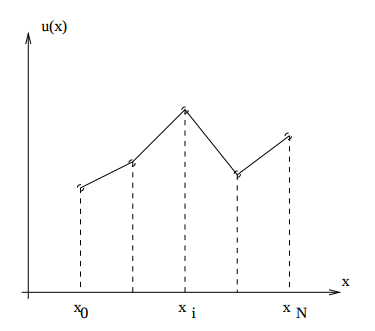
\includegraphics[width=0.3\textwidth]{img/19/fin_elem_method}
		\end{figure}
		
		\begin{itemize}
			\item odcinek $[x_0, x_N] \rightarrow$ podział na N części
			\item na każdym $[x_i, x_{i+1}]$ przybliżamy $\varphi(x)$ przez linię prostą odcinek $[x_i, x_{i+1}] \Rightarrow$
		\end{itemize}
		Element:
		$$
		u^{(i)}(x) = u_i + \frac{x - x_i}{x_{i+1} - x_i}(u_{i+1} - u_i)
		$$
		
		$$
		u_x^{(i)}(x) = \frac{u_{i+1} - u_i}{x_{i+1} - x_i}
		$$
		
	\end{frame}
	
%%%%%%%%%%%%%%%% 
	
	\begin{frame}{Metoda elementu skończonego}
		Przybliżony funkcjonał ma postać:
		
		$$
		I[u] = \sum_{i=0}^{N-1} \int_{x_i}^{x_{i+1}} F(x, u^{(i)}, u_x^{(i)} ) dx
		$$
		
		Stałe $u_i$ należy dobrać tak, by $I[u]$ był ekstremalny, tj.
		
		$$
		\frac{\partial I[u]}{\partial u_i} = 0, i = 1, ... , N-1
		$$
		
		
		\begin{itemize}
			\item liniowa aproksymacja $\Rightarrow$ proste całkowanie
			\item do rozwiązania: układ równań liniowych
			\item uogólnienia: 2D, 3D...
		\end{itemize}
		
		% Dead link 
		% Simple Finite Element - Applet (Jason White)
		% http://mech.utah.edu/~jwhite/assign8/SimpleFE.html
	\end{frame}




